\documentclass{beamer}
\usepackage{algorithm} %pseudo-code
\usepackage{algpseudocode}
\usepackage{amsmath, amssymb, amscd}
\usepackage{graphicx}
\usepackage{float}
\usepackage{amsmath, amssymb, amscd}
\usepackage{alltt}
\usepackage{textcomp}
\usepackage{gensymb}
\usepackage{multicol}
\usepackage{tabularx}

\newcommand{\N}{\mathbb{N}}
\newcommand{\Z}{\mathbb{Z}}
\newcommand{\R}{\mathbb{R}}
\newcommand{\bigo}{\mathcal{O}}
\newcommand{\G}{\mathcal{G}}
\newcommand{\V}{\mathcal{V}}
\newcommand{\E}{\mathcal{E}}
\newcommand{\K}{\mathcal{K}}
\newcommand{\T}{^\intercal}

\newcommand{\sups}[1]{\ensuremath{^{\textrm{#1}}}}
\newcommand{\subs}[1]{\ensuremath{_{\textrm{#1}}}}

\newcommand{\specialcell}[2][c]
{
  \begin{tabular}[#1]{@{}c@{}}#2\end{tabular}
}

\makeatletter
\newsavebox{\mybox}\newsavebox{\mysim}
\newcommand{\distras}[1]
{
  \savebox{\mybox}{\hbox{\kern3pt$\scriptstyle#1$\kern3pt}}%
  \savebox{\mysim}{\hbox{$\sim$}}%
  \mathbin{\overset{#1}{\kern\z@\resizebox{\wd\mybox}{\ht\mysim}{$\sim$}}}%
}
\makeatother
%===============================================================================
% code highlighting :
\usepackage{listings}

% define custom colors :
\usepackage{color}
\definecolor{bg}{rgb}{0.96,0.96,0.85}
\definecolor{deepblue}{rgb}{0,0,0.5}
\definecolor{deepred}{rgb}{0.6,0,0}
\definecolor{deepgreen}{rgb}{0,0.5,0}

\usepackage{xcolor}
\renewcommand{\lstlistlistingname}{Code Listings}
\renewcommand{\lstlistingname}{Code Listing}
\definecolor{gray}{gray}{0.5}
\colorlet{commentcolour}{green!50!black}

\colorlet{stringcolour}{red!60!black}
\colorlet{keywordcolour}{magenta!90!black}
\colorlet{exceptioncolour}{yellow!50!red}
\colorlet{commandcolour}{blue!60!black}
\colorlet{numpycolour}{blue!60!green}
\colorlet{literatecolour}{magenta!90!black}
\colorlet{promptcolour}{green!50!black}
\colorlet{specmethodcolour}{violet}
\colorlet{indendifiercolour}{green!70!white}

\newcommand{\framemargin}{5ex}

\newcommand{\literatecolour}{\textcolor{literatecolour}}

\newcommand\pythonstyle{\lstset{
%keepspaces=true,
language=python,
showtabs=true,
tab=,
tabsize=2,
basicstyle=\ttfamily\scriptsize,%\setstretch{.5},
stringstyle=\color{stringcolour},
showstringspaces=false,
alsoletter={1234567890},
otherkeywords={\ , \}, \{, \%, \&, \|},
keywordstyle=\color{keywordcolour}\bfseries,
emph={and,break,class,continue,def,yield,del,elif ,else,%
except,exec,finally,for,from,global,if,import,in,%
lambda,not,or,pass,print,raise,return,try,while,assert},
emphstyle=\color{blue}\bfseries,
emph={[2]True, False, None},
emphstyle=[2]\color{keywordcolour},
emph={[3]object,type,isinstance,copy,deepcopy,zip,enumerate,reversed,list,len,dict,tuple,xrange,append,execfile,real,imag,reduce,str,repr},
emphstyle=[3]\color{commandcolour},
emph={Exception,NameError,IndexError,SyntaxError,TypeError,ValueError,OverflowError,ZeroDivisionError},
emphstyle=\color{exceptioncolour}\bfseries,
%upquote=true,
morestring=[s]{"""}{"""},
morestring=[s]{'''}{'''},
commentstyle=\color{commentcolour}\slshape,
%emph={[4]1, 2, 3, 4, 5, 6, 7, 8, 9, 0},
emph={[4]ode, fsolve, sqrt, exp, sin, cos, arccos, pi,  array, norm, solve, dot, arange, , isscalar, max, sum, flatten, shape, reshape, find, any, all, abs, linspace, legend, quad, polyval,polyfit, hstack, concatenate,vstack,column_stack,empty,zeros,ones,rand,vander,grid,pcolor,eig,eigs,eigvals,svd,qr,tan,det,logspace,roll,min,mean,cumsum,cumprod,diff,vectorize,lstsq,cla,eye,xlabel,ylabel,squeeze,plot,median,std,hist},
emphstyle=[4]\color{numpycolour},
emph={[5]__init__,__add__,__mul__,__div__,__sub__,__call__,__getitem__,__setitem__,__eq__,__ne__,__nonzero__,__rmul__,__radd__,__repr__,__str__,__get__,__truediv__,__pow__,__name__,__future__,__all__},
emphstyle=[5]\color{specmethodcolour},
emph={[6]assert,range,yield},
emphstyle=[6]\color{keywordcolour}\bfseries,
% emph={[7]self},
% emphstyle=[7]\bfseries,
literate=*%
{:}{{\literatecolour:}}{1}%
{=}{{\literatecolour=}}{1}%
{-}{{\literatecolour-}}{1}%
{+}{{\literatecolour+}}{1}%
{*}{{\literatecolour*}}{1}%
{/}{{\literatecolour/}}{1}%
{!}{{\literatecolour!}}{1}%
%{(}{{\literatecolour(}}{1}%
%{)}{{\literatecolour)}}{1}%
{[}{{\literatecolour[}}{1}%
{]}{{\literatecolour]}}{1}%
{<}{{\literatecolour<}}{1}%
{>}{{\literatecolour>}}{1}%
{>>>}{{\textcolor{promptcolour}{>>>}}}{1}%
,%
breaklines=true,
breakatwhitespace= true,
%xleftmargin=\framemargin,
%xrightmargin=\framemargin,
aboveskip=1ex,
frame=trbl,
%frameround=tttt,
rulecolor=\color{black!40},
%framexleftmargin=\framemargin,
%framextopmargin=.1ex,
%framexbottommargin=.1ex,
%framexrightmargin=\framemargin,
%framexleftmargin=1mm, framextopmargin=1mm, frame=shadowbox, rulesepcolor=\color{blue},#1
%frame=tb,
backgroundcolor=\color{yellow!10}
}}

% Python environment
\lstnewenvironment{python}[1][]
{
  \pythonstyle
  \lstset{#1}
}
{}

% Python for external files
\newcommand\pythonexternal[1]
{{
  \pythonstyle
  \lstinputlisting{#1}
}}

% Python for inline
\newcommand\pythoninline[1]{{\pythonstyle\lstinline!#1!}}

% end code highlighting
%===============================================================================


\begin{document}
\small

\title{Killer Yeast Vs. Sensitive Yeast}
\author{Evan Cummings \and Intizor Aliyorov \and Malachi J.\ Cryder\\
MATH 445 - Statistical, Dynamical, and Computational Modeling}

\maketitle

\section*{Proposal}
The differential equation we may use for modeling the growth of yeast is the same as that used for bacterial growth in a chemostat:
\begin{align*}
  \frac{dN}{dt} &= k(C) N - \frac{FN}{V}, \\
  \frac{dC}{dt} &= -\alpha k(C) N - \frac{FC}{V} + \frac{FC_0}{V},
\end{align*}
with initial conditions $C(0) = C_i$ and $N(0) = N_i$, $N$ is the number of yeast in the chamber in units number/volume, $C$ is the concentration of nutrient in the chamber with units mass/volume, $C_0$ is the concentration of nutrient in the reservoir, $F$ is the in/out flow rate with units volume/time, $V$ is the volume of the chamber, $\alpha$ is a unitless inverse of the yield constant, and $k(C)$ is the reproduction rate for yeast in units 1/time with possible formula chosen such that $\lim_{C \rightarrow \infty} = k_{max}$, and $k_{max}$ represents the maximum possible reproduction rate:
$$k(C) = \frac{k_{max} C}{k_n + C}.$$
where $k_n$ is chosen such that $k(k_n) = k_{max} / 2$.  The quantitative measurement for fitness is a measurement of optical density at steady state (equilibrium) at a given flow rate ($F$) in volumes/hr.

Because the data is collected in density form, we propose solving for density $\rho = N/V$:
\begin{align*}
  \frac{d\rho}{dt} &= k(C) \rho - \frac{F\rho}{V}, \\
  \frac{dC}{dt} &= -\alpha k(C) \rho - \frac{FC}{V} + \frac{FC_0}{V},
\end{align*}
with initial conditions $\rho(0) = \rho_i$ and $C(0) = C_i$, and all other constants are identical as before.

In order to find the steady states, we have to find the intersections of the null-clines at equilibrium points $(\bar{\rho}, \bar{C})$, i.e.\ $d\bar{\rho}/dt = 0$ and $d\bar{C}/dt = 0$:
\begin{align*}
  \frac{d\rho(\bar{\rho}, \bar{C})}{dt} &= k(\bar{C}) \bar{\rho} - \frac{F\bar{\rho}}{V}, \\
  &= \bar{\rho} \left( k(\bar{C}) - \frac{F}{V} \right) = 0, \\
\end{align*}
which is zero for $\bar{\rho} = 0$ or $k(\bar{C}) = F/V$.  Solving the other equation gives us the other steady-states:
\begin{align*}
  \frac{dC(\bar{\rho}, \bar{C})}{dt} &= -\alpha k(\bar{C}) \bar{\rho} - \frac{F\bar{C}}{V} + \frac{FC_0}{V} = 0,
\end{align*}
which is zero for $\alpha k(\bar{C}) \bar{\rho} + \frac{F\bar{C}}{V} = \frac{FC_0}{V}$.

In order to evaluate these null-clines, we need to evaluate the non-trivial cases, here for $\dot{\rho} = 0$,
\begin{align}
  k(\bar{C}) = \frac{k_{max} \bar{C}}{k_n + \bar{C}} &= \frac{F}{V} \notag \\
  k_{max} \bar{C} &= \frac{F}{V} (k_n + \bar{C}) \notag \\
  k_{max} \bar{C} - \frac{F}{V}\bar{C} &= \frac{F}{V} k_n \notag \\
  \bar{C} \left( k_{max} - \frac{F}{V} \right) &= \frac{F}{V} k_n \notag \\
  \bar{C} &= \frac{F k_n}{V \left( k_{max} - \frac{F}{V}\right)} \notag \\
  \bar{C} &= \frac{F k_n}{V k_{max} - F}.
\end{align}
Likewise, for $\dot{C} = 0$,
\begin{align}
  \alpha k(\bar{C}) \bar{\rho} + \frac{F\bar{C}}{V} &= \frac{FC_0}{V} \notag \\
  \alpha \left[ \frac{k_{max}\bar{C}}{k_n + \bar{C}} \right] \bar{\rho} + \frac{F\bar{C}}{V} &= \frac{FC_0}{V} \notag \\
  \alpha k_{max}\bar{C} \bar{\rho} + \frac{F\bar{C}}{V} (k_n + \bar{C}) &= \frac{FC_0}{V} (k_n + \bar{C}) \notag \\
  \alpha k_{max}\bar{C} \bar{\rho} + \frac{F\bar{C}}{V} (k_n + \bar{C}) &= \frac{FC_0}{V} (k_n + \bar{C}) \notag \\
  \alpha k_{max}\bar{C} \bar{\rho} + \frac{F\bar{C} k_n}{V} + \frac{F\bar{C}^2}{V}  &= \frac{FC_0 k_n}{V} + \frac{FC_0 \bar{C}}{V} \notag \\
  \alpha k_{max}\bar{C} \bar{\rho} &= \frac{FC_0 k_n}{V} + \frac{FC_0 \bar{C}}{V} - \frac{F\bar{C} k_n}{V} - \frac{F\bar{C}^2}{V} \notag \\
  \bar{\rho} &= \frac{FC_0 k_n}{V(\alpha k_{max} \bar{C})} + \frac{FC_0 \bar{C}}{V(\alpha k_{max} \bar{C})} - \frac{F\bar{C} k_n}{V(\alpha k_{max} \bar{C})} - \frac{F\bar{C}^2}{V(\alpha k_{max} \bar{C})} \notag \\
  \bar{\rho} &= \frac{FC_0 k_n}{V \alpha k_{max} \bar{C}} + \frac{FC_0}{V \alpha k_{max}} - \frac{F k_n}{V \alpha k_{max}} - \frac{F\bar{C}}{V \alpha k_{max}} \notag \\
  \bar{\rho} &= \frac{F}{V \alpha k_{max}} \left( \frac{C_0 k_n}{\bar{C}} + C_0 - k_n - \bar{C} \right). 
\end{align}

\newpage

\begin{multicols}{2}
\begin{figure}[H]
  \centering
    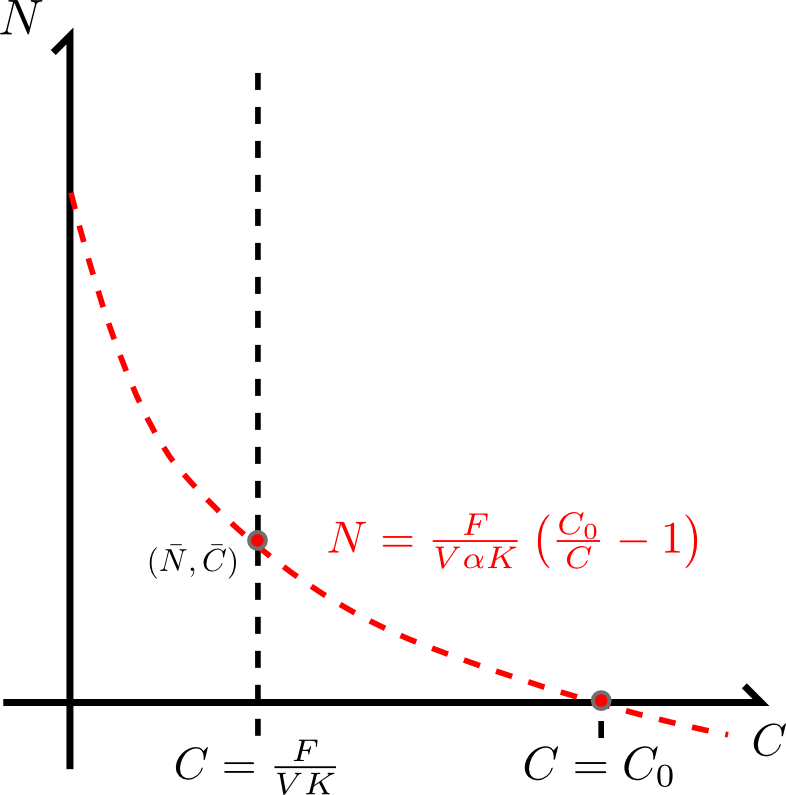
\includegraphics[width=0.40\textwidth]{images/drawing.png}
  \caption{\footnotesize The $\dot{C} = 0$ nullcline (red) intersecting with the $\dot{\rho} = 0$ nullcline (black).  The trivial steady-state $(0,0)$ and non-trivial steady-state $(\bar{\rho}, \bar{C})$ are shown as red dots.}
\end{figure}
\vfill
\columnbreak
By placing Eq.\ (1) inside Eq.\ (2), we can find the intersection of the null-clines:
\scriptsize
\begin{align*}
  \bar{\rho}(\bar{C}) &= \frac{F}{V \alpha k_{max}} \left( \frac{C_0 k_n}{\bar{C}} + C_0 - k_n - \bar{C} \right) \\
  &= \frac{F}{V \alpha k_{max}} \left( \frac{C_0 k_n}{\frac{F k_n}{V k_{max} - F}} + C_0 - k_n - \frac{F k_n}{V k_{max} - F} \right) \\
  &= \frac{F}{V \alpha k_{max}} \left( \frac{C_0(V k_{max} - F)}{F} + C_0 - k_n - \frac{F k_n}{V k_{max} - F} \right).
\end{align*}
\small
The unknowns in this are $\alpha$, $k_{max}$, and $k_n$.  First, assume $\alpha = 1$.  With this assumption we can then minimize the difference between the equilibrium solution for $\rho$ determined from the differential equations $\dot{\rho}$ and $\dot{C}$ (determined numerically) and the observed optical density $\bar{\rho}$ for a given $F$ to provide an estimate for $\bar{C}$, which we can then plug into equations (1) and (2) to get $k_{max}$ and $k_n$.
\end{multicols}

The data we are provided with include two sets of two separate runs, along with the concentration of nutrient in the reservoir, $C_0 = 0.02$:
\section{K1 Run}
\subsection*{Vessel One :}
\begin{center}
\begin{tabular}{l|cccccccc}
  Volumes/Hr & 0.028 & 0.099 & 0.142 & 0.207 & 0.269 & 0.287 & 0.352 & 0.403 \\
  Optical Density at Steady State & 0.144 & 0.151 & 0.099 & 0.069 & 0.045 & 0.02 & 0.003 & 0 \\
\end{tabular}
\end{center}

\subsection*{Vessel Two :}
\begin{center}
\begin{tabular}{l|ccccccccc}
  Volumes/Hr & 0.054 & 0.11 & 0.141 & 0.199 & 0.257 & 0.296 & 0.348 & 0.397 & 0.41 \\
  Optical Density at Steady State & 0.164 & 0.151 & 0.11 & 0.092 & 0.072 & 0.023 & 0.006 & 0.002 & 0.004 \\
\end{tabular}
\end{center}

\section{Sensitive Run}
\subsection*{Vessel One :}
\begin{center}
\begin{tabular}{l|ccccccccc}
  Volumes/Hr & 0.041 & 0.099 & 0.167 & 0.223 & 0.266 & 0.328 & 0.356 & 0.401 & 0.462 \\
 Optical Density at Steady State & 0.54 & 0.494 & 0.459 & 0.395 & 0.229 & 0.019 & 0.006 & 0.003 & 0  \\
\end{tabular}
\end{center}

\subsection*{Vessel Two :}
\begin{center}
a\begin{tabular}{l|ccccccc}
 Volumes/Hr & 0.0571 & 0.126 & 0.196 & 0.263 & 0.313 & 0.383  \\
  Optical Density at Steady State & 0.385 & 0.456 & 0.363 & 0.197 & 0.044 & 0.004 \\
\end{tabular}
\end{center}


\begin{figure}[H]
  \centering
    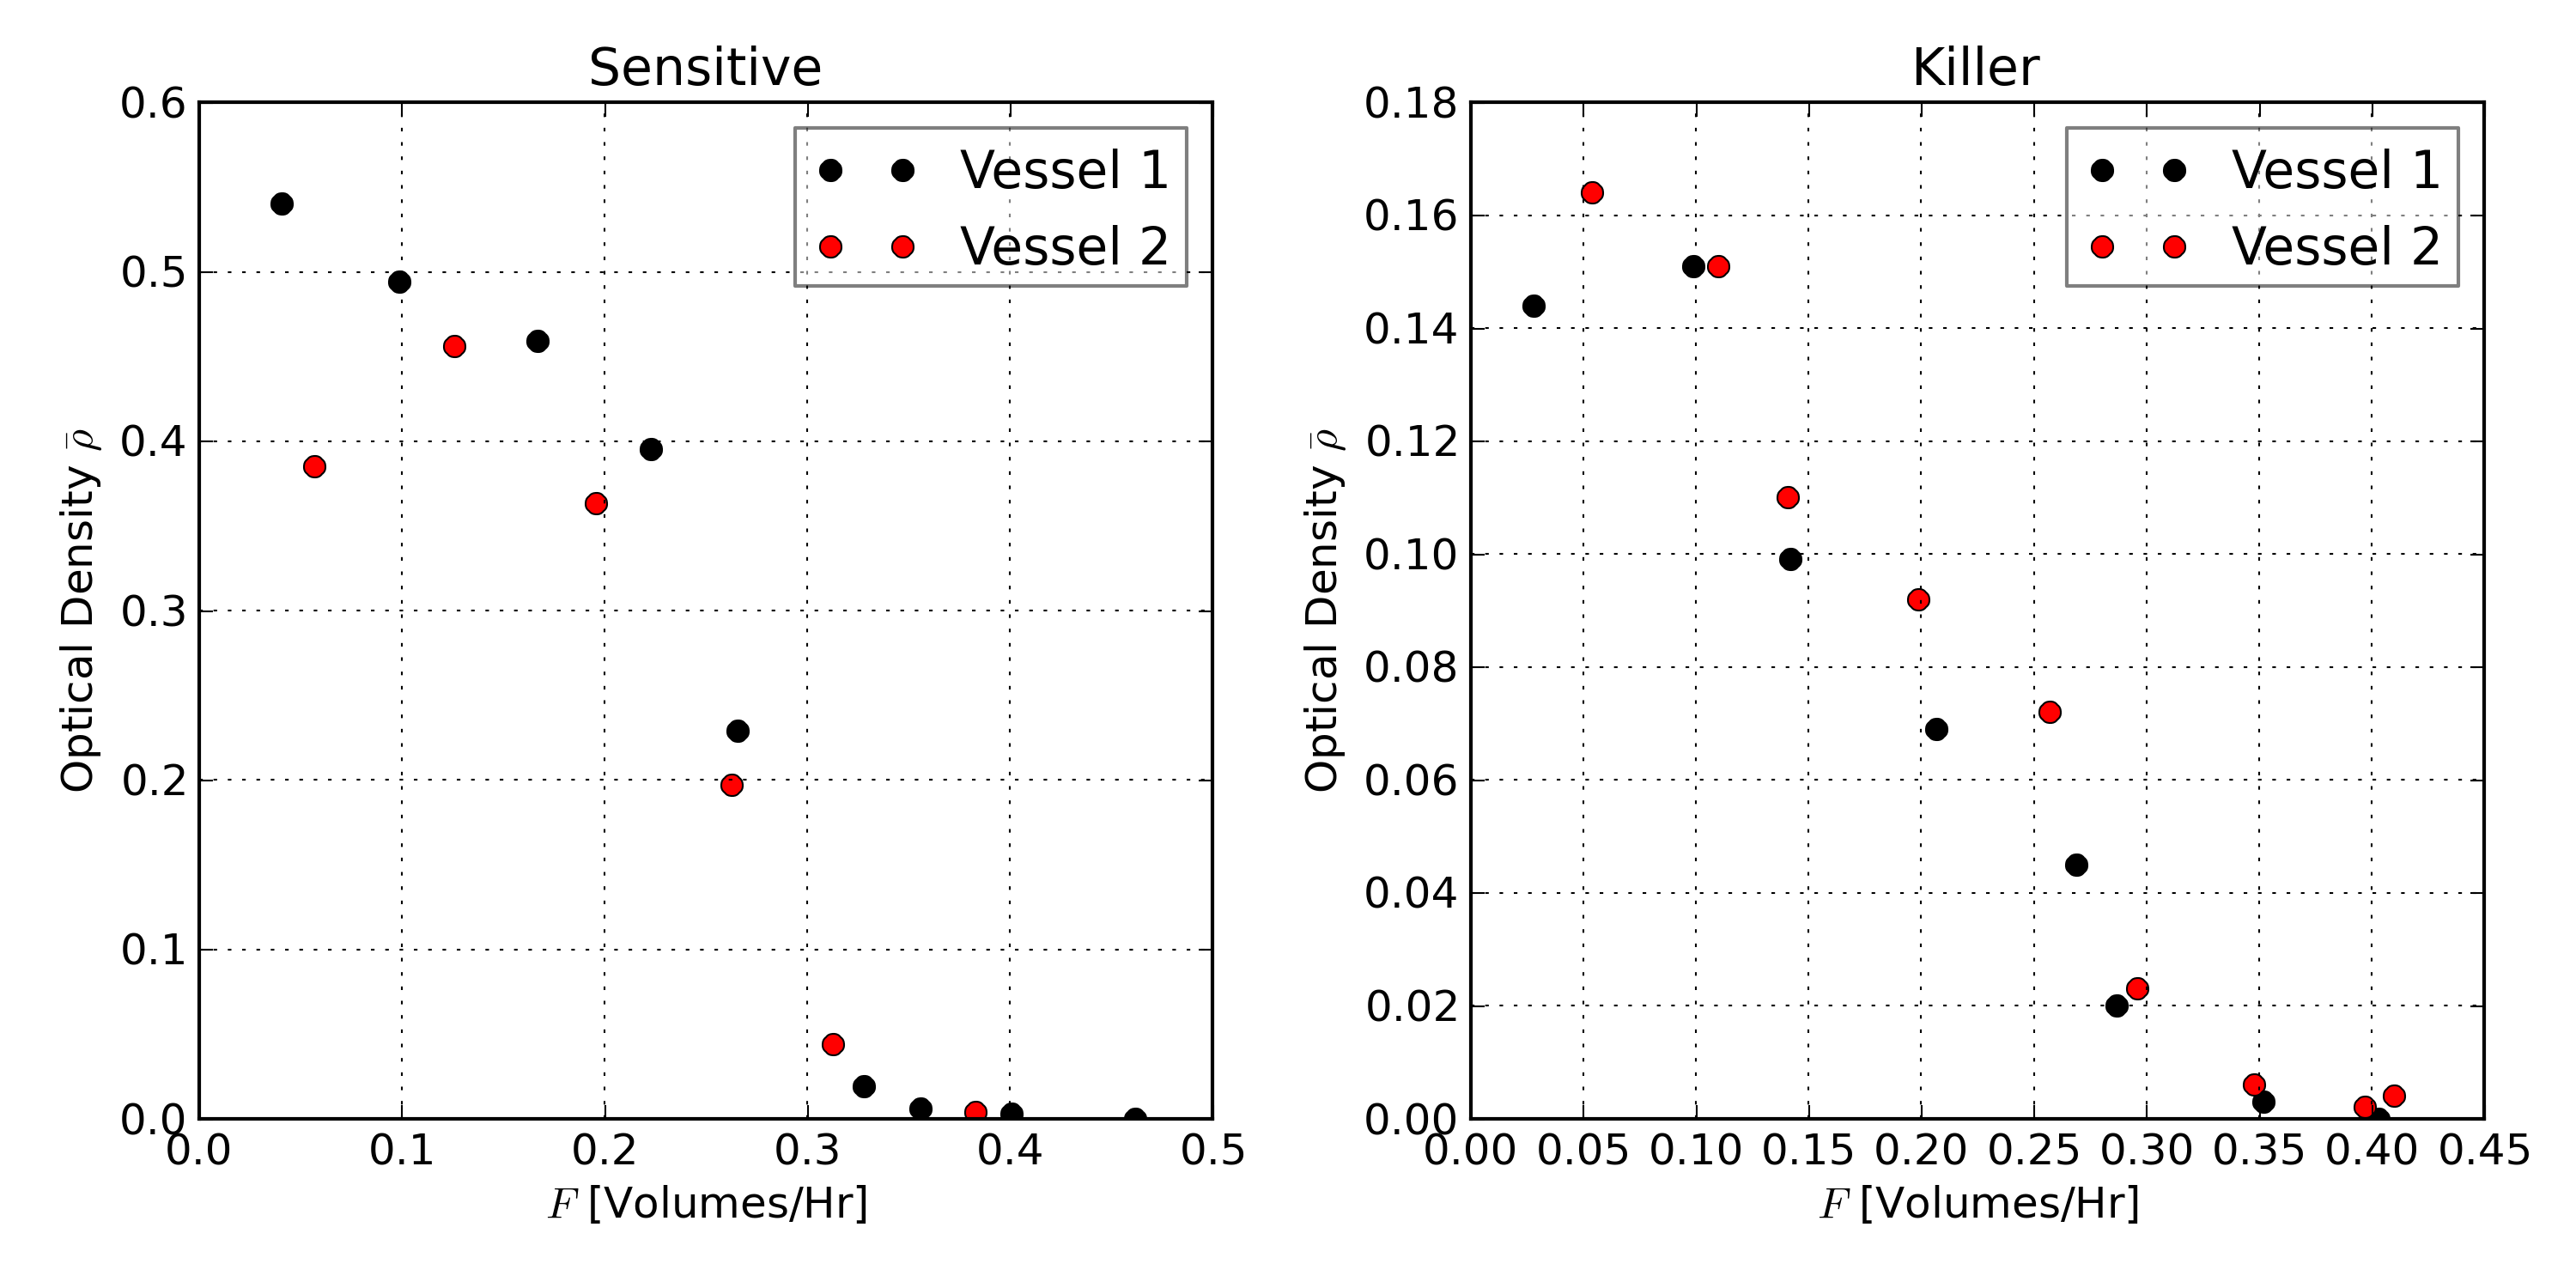
\includegraphics[width=1.0\textwidth]{images/data.png}
\end{figure}

\end{document}


